\documentclass[letterpaper, twoside, 12 pt]{article}
\usepackage{james_kj}

% Use this to toggle professionalism
\newif\ifpresstime
\presstimefalse
\presstimetrue

\ifpresstime
	\renewcommand{\meo}[1]{}
\fi

\tikzset{
	pointer/.style={->, >= stealth, shorten <= 7 pt, shorten >= 2 pt}
}

\title{The Kutta--Joukowski Theorem}
\date{\today}
\author{James McFeeters}
\begin{document}
	\maketitle
	\newcounter{y}
	\setcounter{y}{0}

\begin{abstract}
	This will be an abstract in the future. 
\end{abstract}

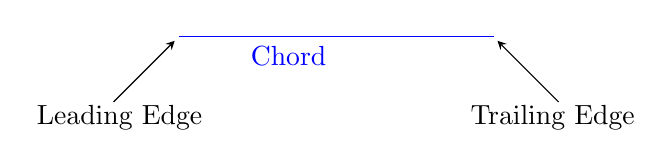
\begin{tikzpicture}
	\newcounter{scale}
	\setcounter{scale}{4}
	\draw[scale = \thescale] node [left=0.5 cm] {} plot file{../airfoils/NACA_0030.dat} -- cycle;

	\draw [blue] (0.0, 0.0) to [out=0, in=180] coordinate[pos=0.1] (1) coordinate[pos=0.5] (2)  coordinate[pos=0.9] (3) (\thescale, 0);
	\node [below left, blue] at (2) {Chord};
	\draw[pointer] (-1, -1) -- node[near start, below]{Leading Edge} (0, 0);
	\draw[pointer] (\thescale + 1, -1) -- node[near start, below]{Trailing Edge} (\thescale, 0);
\end{tikzpicture}

\clearpage
\nocite{*}
\bibliographystyle{plainnat}
\bibliography{kj_references}

\end{document}
